%%%%%%%%%%%%%%%%%%%%%%%%%%%%%%%%%%%%%%%%%%%%%%%%%%%%%%%%%%%%%%%%%%%%%%%%
%                                                                      %
%     File: Thesis_Introduction.tex                                    %
%     Tex Master: Thesis.tex                                           %
%                                                                      %
%     Author: Andre C. Marta                                           %
%     Last modified :  2 Jul 2015                                      %
%                                                                      %
%%%%%%%%%%%%%%%%%%%%%%%%%%%%%%%%%%%%%%%%%%%%%%%%%%%%%%%%%%%%%%%%%%%%%%%%
\newcommand{\SubItem}[1]{
	{\setlength\itemindent{15pt} \item[-] #1}
}

\theoremstyle{definition}
\newtheorem{definition}{Definition}[section]

\chapter{Introduction}
\label{chapter:introduction}

In this chapter, the motivation behind the work is introduced, as well as the problem and the objectives to be achieved. 



%%%%%%%%%%%%%%%%%%



%%%%%%%%%%%%%%%%%%%%%%%%%%%%%%%%%%%%%%%%%%%%%%%%%%%%%%%%%%%%%%%%%%%%%%%%
\section{Motivation}
\label{section:motivation}


Given the complexity of modern software systems, it is increasingly crucial to maintain quality and reliability, in a time-saving and cost-effective manner, specially in large and fast-paced companies. This is why many industries adopt a \textit{Continuous Integration} (CI) strategy, which is a popular software development technique where engineers, frequently, incorporate code changes into the mainline codebase, allowing them to easily check that their code can build successfully and pass tests across various system environments \cite{santolucito2018statically} . The latter task performed in the process is called \textit{regression testing}. To ensure that the introduction of new features or the fix of known failures not only are correct, but also do not obstruct existing functionalities. Ergo, regression testing plays a fundamental role on certifying that newer versions adhere to the mainline.  
\par Regression can have many origins, namely code does not compile, performance drops or tests fail, and, as software teams grow, due to the rising amount of changes , the probability that one  creates a conflict is significant. Identifying and amending such regressions constitutes one of the most challenging, costly and time-consuming tasks in the software development life-cycle \cite{Ziftci}.
\par In the last decades, there has been a high demand for automated techniques that accelerate early fault detection, minimizing human intervention. Regression test prioritization lies at the core of these techniques, as one of the most thriving fields in achieving promising results, with increasing research attention (reference). Aiming to find the optimal permutation of ranked tests that match a certain criteria, i.e. the ability to detect faults \text{a priori}, the likelihood a change has of being merge and/or a limited time-frame  \cite{palma}. 
\par The automation process is accomplished through developing algorithms that are, traditionally, programmed for a certain objective, by obeying a set of well-defined instructions. Many traditional algorithms may have shortcomings and not scale well with the complexity of today's systems. However, in recent years, the field of Artificial Intelligence as been expanding at an astounding pace, fueled by the growth of computer power and the amount of available data. In particular, there is a trend in capitalizing machine learning (ML) algorithms and data-driven approaches to solve these kind of problems  \cite{durelli} . 
\par Concretely, in a supervised learning task, given a code change and a list of test cases to be prioritized, test cases can be classified as "pass" or "fail", depending on some set of features and use the result to rank failing tests first.
In fact, Catal \cite{catal} showed that ML approaches can improve the probability of fault detection, when compared to classic software algorithms. 
Powerful results have been achieved by several authors: Chen et al. \cite{chen} use semi-supervised K-Means to cluster test cases and then pick a small subset of tests from each cluster, Uber developers \cite{Uber} built a speculation engine powered by Logistic regression to predict failed test cases and more recently, Palma et al. \cite{palma} combined traditional test and similarity-based quality metrics, and Lachmann et al. \cite{lachmannlp} resorted to textual information to extract features from test descriptions written in Natural Language.


\section{Version Control Systems}

In software engineering, version control systems are a mean of keeping track of incremental versions of files and documents. Allowing the user to arbitrarily explore and recall the past changes that lead to that specific version. Usually in these kind of systems, changes are uniquely identified, either by a code number or letter, an associated timestamp and the author.\cite{santolucito2018statically} 

%%%%%%%%%%%%%%%%%%

\subsection{Repository \& Working Copy}

The central piece of these systems is the \textbf{Repository}. - which is the data structure where all the current and historical files are stored and possibly, remotely, accessible to others (\textit{clients}).\cite{santolucito2018statically} When a client \textit{writes} information, it becomes accessible to others and when one \textit{reads}, obtains information from the repository. The major difference from an usual server is the capability of remembering every version of the files. With this formulation, a client has the possibility to request any file from any previous version of the system.
\par While developing, having multiple versions of a project is not very useful, given that most compilers only know how to interpret one code version with a specific file type. So the bridge linking the repository and the user is the \textbf{working copy}. - a local copy of a particular version, containing files or directories, on which the user is free to work on and later on communicate the changes to the repository.\cite{santolucito2018statically}

%%%%%%%%%%%%%%%%%%

\section{Mono-repositories vs. Multi-repositories}
%reformulate everything

In order to manage and store amount of new code produced daily, there are two possible ways of organizing repositories: one single giant repository that encompasses every project or assigning one repository for each one. Google's strategy is to store billions of lines of code in one single giant repository, rather than having multiple repositories. \cite{Potvin:2016:WGS:2963119.2854146}
A mono-repository is defined such that it encompasses the following properties: 
\begin{itemize}
	\item \textbf{Centralization} - one code base for every project.
	\item \textbf{Visibility} - Code accessible and searchable by everyone.
	\item \textbf{Synchronization} - Changes are committed  to the mainline.
	\item \textbf{Completeness} - Any project in the repository can only be built from dependencies that are also part of it. 
	\item \textbf{Standardization} - developers communalize the set of tools and methodologies to interact with code.
\end{itemize}

This gives, the vast number of developers working at Google, the ability to access a centralized version of the code base - \textit{"one single source of truth"}, foment code sharing and recycling, increase in development velocity,  intertwine dependencies between projects and platforms, encourage cross-functionality in teams, broad boundaries regarding code ownership, enhance code visibility and many more. However, giant repositories may imply less autonomy and more compliance to the tools used and the dependencies between projects. Also developers claim to be overwhelmed by its size and complexity.
\par A multi-repository is one where the code is divided by projects. With the advantages that engineers can have the possibility of choosing, with more flexibility, the tools/methodologies with which they feel more at ease; the inter dependencies are reduced, providing more code stability, possibly accelerating development. However, the major con arises from the lack of necessity of synchronization, causing version problems and inconsistencies, for example two distinct projects that rely on the same library.
\par Although electing a preferred candidate is still a matter of debate, mono-repositories are linked to less flexibility and autonomy when compared to multi-repositories, but there is the gain of consistency, quality and also the culture of the company is reinforced, by unifying the tools used to link the source code to the engineer.\cite{Jaspan:2018:ADM:3183519.3183550}


\section{Continuous Integration}

In this section, the goal is to provide a solid comparison between the different strategies that can be adopted to make sure source-code repositories are a manageable choice.

%-----------------------------------
%	SUBSUBSECTION 1
%-----------------------------------

\subsection{CI Approaches}

\subsubsection{Naive-approach}

The simplest approach is to run every test for every single commit. As teams get bigger,  both the number of commits and the numbers of tests grow linearly, so this solution does not scale. Also, as \cite{Memon:2017:TGC:3103112.3103143} stated, computer resources grow quadratically with two multiplicative linear factors, making continuous integration a very expensive and not eco-friendly process in terms of resources and time.
\par For example, Google's source code is of the order of 2 billion lines of code and, on average, 40000 code changes are committed daily to Google's repository, adding to 15 million lines of code, affecting 250000 files every week, having the need to come up with new and innovative strategies to handle the problematic.\cite{Ziftci}


%-----------------------------------
%	SUBSUBSECTION 2
%-----------------------------------

\subsubsection{Cumulative Approach}

One possible solution to contour the large amount of time spent on testing and waiting for results is to accumulate all the commits made during working hours and test the last version, periodically, lets say during the night. This enables teams to develop at a constant speed without having the concern of breaking the master branch, but rather worrying about it in the future. In this case, the lag between making a commit and knowing if it passed or fail is very large, running the risk of stacking multiple mistakes on top of each other. 
\par Using this approach, two possible outcomes can occur: either the build passes every test and the change is integrated, or it fails, causing a regression. Here, we encounter another crossroads, as the batch was tested as a cumulative result, we have no information whatsoever of what commit, exactly, caused the regression. This problem can be solved by applying search algorithms:

\begin{itemize}
	\item \textbf{Binary Search} - instead of running every option, divide the list in half and test the obtained subset, if pass, the mistake is located in the other half, if fail, split the subset and test again until narrowing it down to a specific change, this approach is O(log n) complex.
\end{itemize}

After finding out which commit caused the regression, it can be fixed or rolled back to the version before the change was introduced, meaning that possibly the progress made during that working day has to be scrapped and re-done, postponing deadlines and, at a human level, lowering down motivation, with developers being "afraid" of making changes that will propagate and will only be detected later on, so allowing a large turn-around time may results in critical hampering of productivity.
\par In comparison with naive-approach, cumulative approach is more scalable in the way that it avoids testing every single commit made, only trying to test the last of the day, spending more time trying to trace back the origin of the failure. So in conclusion, we forfeit absolute correctness to gain speed and pragmatism, although this solution's computer resources grow linearly with the number and time of tests. 
\par The key is that we should be able to go beyond finding items in a list were elements are interchangeable and equally informative. We should be able to use that information to do a much more efficient search. For example, we are looking for a faulty commit in a list of 10 elements and we know with a 95$\%$ probability that the commit is one of the last 4 elements, then we should only do binary search on those 4, instead of 10, thus saving time.

%-----------------------------------
%	SUBSUBSECTION 3
%-----------------------------------

\subsubsection{Change-List Approach}

In this case, changes are compiled and built in a serialized manner, each change is atomic and denoted as a Change List (CL). Clarifying, lets take a look at Google's example of workflow in Figure \ref{googleWF}.

\begin{figure}[H]
	\centering
	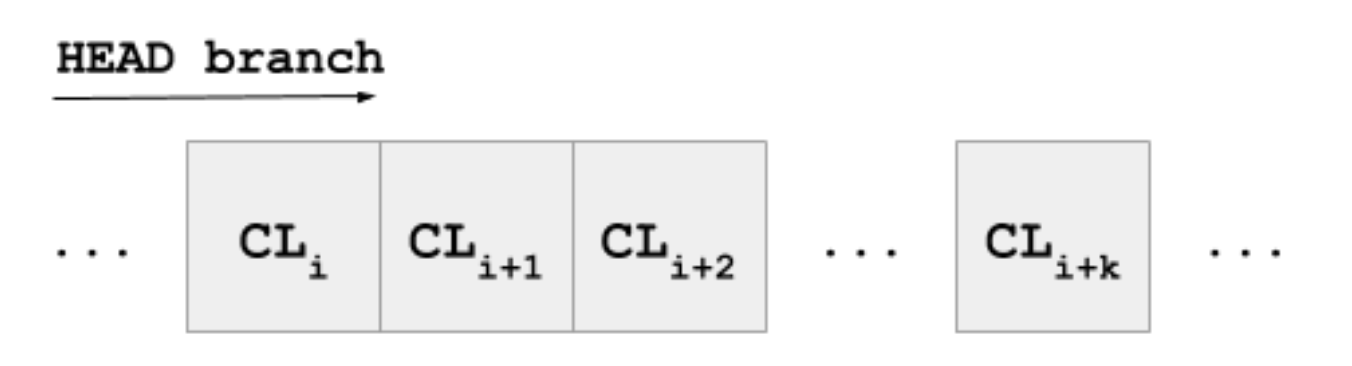
\includegraphics[scale=0.5, width=0.6\linewidth]{figures/Google_WorkFlow.png}
	\caption{Code repository and workflow at Google. Each CL is submitted to master branch or HEAD \cite{Ziftci}}
	\label{googleWF}
\end{figure} 

Individually, tests validate each CL and if the outcome is pass, the change is incorporated into the master branch, resulting into a new version of the code. Otherwise, a regression is caused. For example, imagine that $CL_i$ introduces a regression, causing failure on the consecutive system versions. Possible fixes and tips: investigate the modifications in $CL_i$, to obtain clues about the root cause of the regression; Debug the fail tests at $CL_i$, which is preferable to debug at later version $CL_{i+k}$, whereas after $CL_i$ code volume might increase or mutate, misleading conclusions; revert or roll back the repository, until the point where it was "green", in this case $CL_{i-1}$.\cite{Ziftci}


The novelty is introduced in test validation: 

\begin{itemize}
	\item \textbf{Presubmit tests} - Prior to CL submission, preliminary relevant small/medium tests are run, if all pass the submission proceeds, else it gets rejected. So instead of having to wait until all tests are complete, the developer has a quick estimate of the status of the project.
	\item \textbf{Postsubmit tests} - After CL submission, large/enormous tests are executed and if they indeed cause a regression, we are again in the situation where we have to find exactly what CL broke the build and, possibly, proceed in the same manner as Cumulative Approach to detect what version caused the regression. \cite{Ziftci}
\end{itemize}

Nevertheless there are some major issues: while presubmit testing, the sole focus is to detect flaws on individual changes and not on concurrent one. \textit{Concurrency} is the term referred to builds that run in parallel with each other, meaning that 2 developers can be committing changes of the same file, that are in conflict with each other, or with other files. Therefore, after precommit phase, there is the need to check all the affected dependencies of every commit, quickly identify were the conflict emerged and eventually roll back in the case of a red master, which can only be done in postcommit stage \cite{Uber} and when a postcommit test fails: a 45 minute test, can potentially take 7.5 hours to pinpoint which CL is faulty, given a 1000 CL search window, so automation techniques, quickly putting them to work and returning to a green branch is pivotal. \cite{Ziftci}
\par To better understand the concept of concurrency and the implications it brings, lets consider there are $n$ concurrent changes in a batch, where all of them pass precommit phase: (1) committing changes 1 to $n-1$ do not lead to breakage, (2) applying the $n^{th}$ change does not break the master, and (3) putting all the changes together breaks the mainline. Which might indicate that  the $n^{th}$ change is in conflict with the rest. Concurrency is practically unavoidable and it is more likely to happen when parts of the code that are interconnected are being altered. Frequent mainline synchronization is a possible path to diminish this effect, forcing developers to always work on the most updated version.\cite{Uber} 

%-----------------------------------
%	SUBSUBSECTION 4
%-----------------------------------

\subsubsection{Always Green Master Approach}

After steering clear of analysing every single change with every single test, or accumulating all the changes and testing them , splitting it into smaller individualized chunks, cherry-picking an ideal and non-redundant subset of tests, prioritizing them by size making it possible to divide test phase into precommit and postcommit, and enabling a status estimate of the likelihood of regressions,   \cite{Uber} proposes that an always green mainline is the priority condition, so that productivity is not hampered. To guarantee an always green master, Uber designed a scalable tool called \textit{SubmitQueue}, where every change is enqueued, tested and, only later on, integrated in the mainline branch if it is safe. The interesting aspect is which changes get tested first, while ensuring serializability. Uber resorts to a probabilistic model that can speculate on the likelihood of a given change to be integrated. - i.e. pass all build steps. Additionally, to agilize this process this service contains a \textit{Conflict Analyzer} to trim down concurrent dependencies. 

\paragraph{Probabilistic Speculation} 

Based on a probabilistic model, powered by logistic regression, it is possible to have an estimate on the outcome a given change will have and with that information select the ones that are more likely to succeed, although other criteria might be chosen. \par
To select the more likely to succeed changes, this mechanism builds a \textit{speculation tree}, which is a binary decision tree. Imagine a situation where two changes, $C_1$ and $C_2$, need to be integrated in the master branch $M$. $C_1$ is merged into $M$ is denoted by $M \oplus C_1$ and the build steps for that change are denoted by $B_1$. $B_{12}$ represents builds for $M \oplus C_1 \oplus C_2 $.  Speculating that $B_1$ has high probability of being integrated, it is useful to test it in parallel with $B_{12}$, because if the assumption is correct, $C_1$ is integrated and now this result can be used to determine if $C_2$ also passes, without testing each one individually and then together. If the speculation is not correct, $C_1$ is not merged and $C_2$ has to build separately by running $B_2$. In the case of three pending changes $C_1$,$C_2$ and $C_3$, the speculation tree is of the form of Figure \ref{spectree}. 

\begin{figure}[H]
\centering
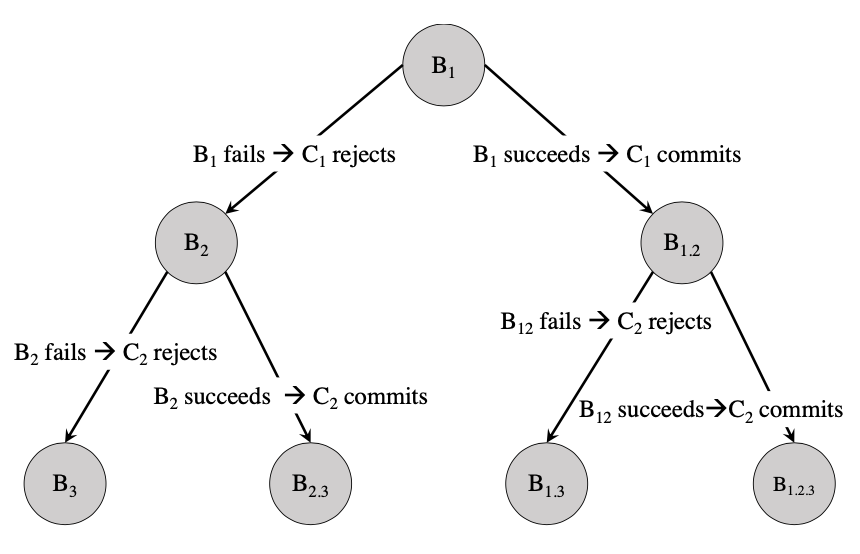
\includegraphics[scale=0.5, width=0.8\linewidth]{figures/spectree.png}
\caption{Speculation tree - builds and outcomes \cite{Uber}}
\label{spectree}
\end{figure}

One possible way of handling the result from this tree would be to speculate everything, assuming that the probability of merging a change is equal to the probability of rejecting it. Having 3 pending changes, one would have to perform 7 builds (number of nodes in the tree), under this assumption. But it is unnecessary to speculate all of the builds, if $B_1$ is successful, $B_2$ now becomes irrelevant and the tree is trimmed down considerably. Only $n$ out of $2^n - 1$ builds are needed to commit $n$ pending changes \cite{Uber}. \par
Additionally, the assumption that every change depends on one another is made, but this is not always the case, two changes can be totally distinct. By detecting independent changes,  a lot of time can be saved by building them individually and committing them in parallel. This is done by the Conflict Analyzer. This approach combining the selection of most likely to pass builds, using machine learning models, parallel execution, the identification of independent changes, trimming down speculation tree size is able to scale thousands of daily commits to a monolithic repository. Finally, a comparison of all explored approaches is shown in the Table below.


\begin{table}[b]
\begin{tabular}{lccc}
	\hline
	\textbf{Approach} & \multicolumn{1}{l}{\textbf{Correctness}} & \textbf{Speed}    & \multicolumn{1}{l}{ \textbf{Scales?}} \\ \hline
	Naive                & Very High                       & Very Low & No                                   \\
	Cumulative           & Medium                          & Low      & No                                   \\
	Change-List          & Medium                            & Medium     & Yes                                  \\
	Always Green Master  & High                            & High     & Yes                                  \\ \hline
\end{tabular}
\caption{Comparative analysis between strategies}
\end{table}


%%%%%%%%%%%%%%%%%%%%%%%%
%%%%%%%%%%%%%%%%%%%%%%%%


\section{Software Testing}

In testing, associated with each repository, there is a battery of tests that makes sure it is safe to integrate a change in the system, but what if we are in the case of applying the same tests twice or more ? What if a test is not adequate to the type of change a developer did? What are the boundaries of test quality? If a test always passes, is it a good test ? Should one apply tests in an orderly way, prioritizing some tests by time or relevance criteria ? 
\par Testing is a verification method to assess the quality of a given software. Although, this sentence is quite valid, it is vague, in the sense that it does not define what quality software actually is. 
In some contexts, quality might just refer to simply code compiling with no syntax errors or "mistakes". When tests are applied, the outcome obtained is of the form PASS/FAIL, with the purpose of verifying functionality or detecting errors, receiving quick and easy to interpret feedback. However, the connections between testing and quality are thin: testing is very much like sticking pins into a doll, to cover its whole surface a lot of tests are needed. For example, running a battery of tests (test suite) where every single one of them yields PASS. This can only mean two things: whether the code is immaculate or some scenarios were left out of the process. Usually, test suites are constructed from failed tests. When in a FAIL situation, i.e. fault detection or removal , a new test case is created, preventing this type of error to slip again in the future, incrementing the existing test suite, in a "never ending" process). 
\par Hence it is correct to say, failed tests are a measure of non-quality, meaning there is no recipe for assuring a software is delivered without flaws.  \cite{7PrinciplesSoftTest}

%-----------------------------------
%	SUBSECTION 4
%-----------------------------------

\subsection{Regression Testing}

Regression testing is performed between two different versions of software in order to provide confidence that the newly introduced features of the working copy do not conflict with the existing features.
In a nutshell, whenever new features are added to an existing software system, not only the new features should be tested, but also the existing ones should be tested to ensure that their behaviours were not affected by the modifications. Usually this is done by applying test cases, to check if those features, in fact work or are still working. Therefore, this field encapsulates the task of managing a pool of tests, that are repeatedly applied across multiple platforms. \cite{ShinThesis} 
\par The problem relies on the fact that tests do not run instantaneously and as software systems become more complex, test pools are ought to grow larger, increasing the cost of regression testing, to a point where it becomes infeasible, due to an elevated consumption of computer and time resources, so there is a high demand to search for automated heuristics that reduce this cost, improving regression testing. In this work, three solutions are proposed that can lead to possible substantial performance improvements:

\begin{itemize}
	\item \textbf{Test Case Selection} - "do smarter" approach, selecting only relevant tests, given the type of change.
	\item \textbf{Test Suite Minimisation} - "do fewer" approach, removing possible redundancies.
	\item \textbf{Test Case Prioritisation} - also "do smarter" approach by running some tests first, increasing probability of early detection. \cite{ShinThesis}
\end{itemize}

In terms of notation, let us denote $P$ as the current version of the program under test, $P'$ as the next
version of $P$. $T$ is the test suite and individual tests are denoted by a lower case letter: $t$. Finally, $P(t)$ is the execution of test $t$ in the system version $P$.


\subsubsection{Test suite minimisation}

\theoremstyle{definition}
\begin{definition}{}
	Given a test suite $T$, a set of test requirements $ R = {r_1, ..., r_n}$ that must be satisfied to yield the desired "adequate" testing, and subsets of T ,  ${T_1, ..., T_n}$, each one associated with the set of requirements, such that any test case $t_j$ belonging to $T_i$ can be used to achieve requirement $r_i$
\end{definition}

The goal is to try to find a subset $T'$ of $T$: $T' \subseteq T$, that satisfies all testing requirements in $R$. A requirement, $r_i$ is attained by any test case, $t_j$ belonging to $T_i$. So a possible solution might be the union of test cases $t_j$ in $T_i$'s that satisfy each $r_i$ (\textit{hitting set}). Moreover, the hitting set can be minimised, to avoid redundancies, this becoming a "minimal set cover problem" or, equivalently, "hitting set problem", that can be represented as a \textit{Bipartite graph}\footnote{s a graph whose vertices can be divided into two disjoint and independent sets $U$ and $V$, such that every edge connects a vertex in $U$ to one in $V$\cite{NPcomplete}}. The minimal hitting-set problem is a NP-complete problem (whose solutions can be verified in polynomial time). \cite{NPcomplete} 
\par Another aspect to consider is that test suite minimisation is not a static process, it is temporary and  it has to be \textit{modification-aware}. - given the type of modification and version of the code, the hitting set is minimised again. \cite{ShinThesis}

\subsubsection{Test Case Selection}


\theoremstyle{definition}
\begin{definition}{}
	Given a program $P$, the version of $P$ that suffered a modification, $P'$, and a test suite $T$, find a subset of $T$, named $T'$ with which to test $P'$.
\end{definition}

Ideally, the choice of $T'$, should contain all the \textit{fault-revealing} test cases in $T$, which are obtained by unveiling the modifications made from $P$ to $P'$. Formally: 

\theoremstyle{definition}
\begin{definition}{\textbf{Modification-revealing test case}}
	A test case $t$ is said to be modification-revealing for $P$ and $P'$ if and only if the output of $P(t) \neq P'(t)$. \cite{Rothermel:1994:FER:257734.257767}
\end{definition}

After finding the nature of the modifications, in simple terms, one has a starting point to select the more appropriate test cases. Both test case minimisation and selection rely on choosing an appropriate subset from the test suite, however they do so, often, with different criteria: in the first case the primal intent is to apply the minimal amount of tests without compromising code coverage in a single version, eliminating permanently the unnecessary tests from the test suite, as in the second the concern is related directly to the changes made from one previous version to the current one. \cite{ShinThesis} 

\subsubsection{Test case prioritisation}

\theoremstyle{definition}
\begin{definition}{}
	Given a test suite $T$, the set containing the permutations of $T$, $PT$, and a function from $PT$ to real numbers $f : PT \rightarrow \mathbb{R}$, find a subset $T'$ such that $(\forall T'')(T'' \in PT)(T'' \neq T')[f(T') \ge f(T'')] $ 
\end{definition}

Where $f$ is a real function that evaluates the obtained subset in terms of a selected criteria: code coverage, early or late fault detection, etc \cite{ShinThesis}. For example, having five test cases (A-B-C-D-E), that detect a total of $10$ faults, there are $5! = 120$ possible ordering, one possible way of choosing a permutation, is to compute the metric Average Percentage of Fault Detection (APFD) \cite{APFD}. 

\theoremstyle{definition}
\begin{definition}{\textbf{APFD}}
	Let $T$ be a test suite containing $n$ test cases and $F$ the set of $m$ faults revealed by $T$. Let $TF_i$ be the order of the first test case that reveals the $i^{th}$ fault.\cite{ShinThesis}
\end{definition}

\begin{equation*}
	APFD = 1 - \frac{TF_{1}+\dots+TF_{n}}{nm} + \frac{1}{2n}
\end{equation*}

Simply, higher values of APFD, imply high fault detection rates, by running few tests, as can be seen in the following plot:

\begin{figure}[h]
	\centering
	f	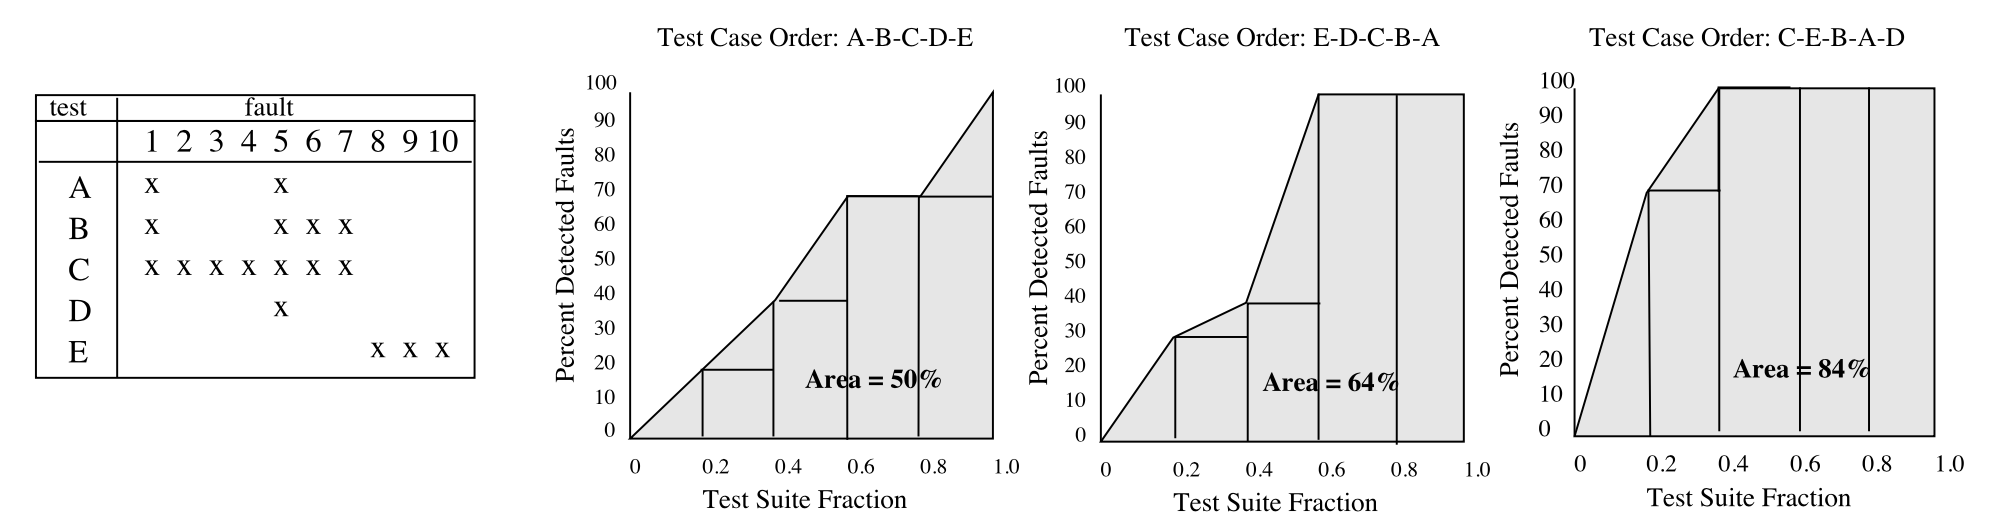
\includegraphics[scale=0.5, width=\linewidth]{figures/APFD.png}
	\caption{Average percentage of fault detection \cite{APFD}}
	\label{APFD}
\end{figure} 

The area below the plotted line is interpreted as the percentage of detected faults against the number of executed test cases, maximizing APFD, demonstrating clear results in detecting early applying fewer test cases. The order of test cases that maximizes APFD, with $ APFD = 84 \%$ is \textbf{C-E-B-A-D}, being preferable over other permutations.
\par By detecting faults early, the risk of developing over faulty code is reduced, causing minimal breakage in productivity avoiding, for example, possible delayed feature releases.\cite{Uber}

%%%%%%%%%%%%%%%%%%%%%%%%%%%%%%%%%%%%%%%%%%%%%%%%%%%%%%%%%%%%%%%%%%%%%%%%

\section{Machine Learning}

Machine Learning algorithms are at the forefront in achieving effective automatic regression testing. By building predictive models, it is possible to accurately, and most importantly, quickly, identify if a newly introduced change is defective or not. This helps developers to check and amend faults, when the details still remain fresh on their minds and it allows to prioritize and organize changes by the risk of being defective, this way testing the ones that are more likely to fail first, diminishing the lag-time between committing and feedback.
\\

In recent years, several researchers studied the usefulness of applying fault-prediction techniques , powered by machine learning algorithms.
More concretely, resorting to an emergent area which is Deep Learning. Kamei et. al propose an approach called \textit{Deeper}, that is divided into two phases: the feature extraction phase and the machine learning phase. The first consist on identifying a combination of relevant features from the initial dataset, by using Deep Belief Networks. The latter is encapsulated on building a classifier/predictive model based on those same features.

In this work, the author aims to replicate and explore the techniques developed by ... and ..., extending the domain of validity and achieving higher levels of accuracy, by experimenting other classifiers and feature extraction techniques.

In the next sections, a theoretical background will be elaborated on the several techniques used throughout the thesis, to provide a solid base for moving forward.

%%%%%%%%%%%%%%%%%%%%%%%%%%%%%%%%%%%%%%%%%%%%%%%%%%%%%%%%%%%%%%%%%%%%%%%%

\section{State of the Art}
\label{section:stateoftheart}

\subsection{Baseline Approaches}

\subsection{Code-Coverage Approaches}

\subsection{History-based Approaches}

\subsection{Modification-based Approaches}


%%%%%%%%%%%%%%%%%%%%%%%%%%%%%%%%%%%%%%%%%%%%%%%%%%%%%%%%%%%%%%%%%%%%%%%%

\section{Test Case Prioritization in Industrial Environments}
\label{section:problem}


What is happening in the current CI system ? numbers of commits per day, number of resources used, amount of data generated, time it takes on average to integrate changes and current "naive  approach"

How is the company expected to grow in the near future ? as teams and projects grow time and resources grow quadratically. 

Consequences of  increasing turn around time: context-loss, productivity hampering, delays. CI aims to  spend less time integrating different developers’ code changes.

trade off speed vs. correctness

%%%%%%%%%%%%%%%%%%%%%%%%%%%%%%%%%%%%%%%%%%%%%%%%%%%%%%%%%%%%%%%%%%%%%%%%


\section{Repository}
\label{section:repository}

For transparency and replication purposes, all the files developed and used throughout this thesis are stored and available to access at  \url{https://github.com/johnnylousas/Master-Thesis}. The online repository contains all open-source datasets,  Python files implemented to apply machine learning and collect results, along with pertinent documentation.

%%%%%%%%%%%%%%%%%%%%%%%%%%%%%%%%%%%%%%%%%%%%%%%%%%%%%%%%%%%%%%%%%%%%%%%%

\section{Objectives \& Thesis Outline}
\label{section:objectives}
Th goal of this thesis is to use Machine Learning pipelines to forecast test case failure likelihood.  
Datasets were algorithms are trained: dummy data (controlled environment) , real-data of BNP (real-world case), OpenSource Data (other datasets available to compare results).
Then for a given revision, choose which chain of test cases minimize pass/fail uncertainty, reducing fault detection time.
Finally, provide a live-estimate of the status of a Project in real time. (farfetched)



The objectives delineated for this work are: 
\begin{itemize}
	\item Detect common usage patterns, in a controlled environment, by generating synthetic data.
	\SubItem{Learn heuristics to automate fault detection process}
	\item Optimize regression testing systems using real world data.
	\SubItem{Analyse how different system configurations affect Continuous Integration}
	\SubItem{Reduce fault detection time}
	\SubItem{Provide a Live-Estimate of the Status of a Project}
	\SubItem{Given a commit, choose which chain of tests minimize pass/fail uncertainty}
\end{itemize}


The thesis is organized as follows: \\
Chapter 2 Background  \\
Chapter 3 Paper 1 \\
Chapter 4 Paper 2 \\
Chapter 5 Conclusions \\  

%%%%%%%%%%%%%%%%%%%%%%%%%%%%%%%%%%%%%%%%%%%%%%%%%%%%%%%%%%%%%%%%%%%%%%%%


